%% (Master) Thesis template
% Template version used: v1.4
%
% Largely adapted from Adrian Nievergelt's template for the ADPS
% (lecture notes) project.


%% We use the memoir class because it offers a many easy to use features.
\documentclass[11pt,a4paper,titlepage]{memoir}

%% Packages
%% ========

%% LaTeX Font encoding -- DO NOT CHANGE
\usepackage[OT1]{fontenc}

%% Babel provides support for languages.  'english' uses British
%% English hyphenation and text snippets like "Figure" and
%% "Theorem". Use the option 'ngerman' if your document is in German.
%% Use 'american' for American English.  Note that if you change this,
%% the next LaTeX run may show spurious errors.  Simply run it again.
%% If they persist, remove the .aux file and try again.
\usepackage[english]{babel}

%% Input encoding 'utf8'. In some cases you might need 'utf8x' for
%% extra symbols. Not all editors, especially on Windows, are UTF-8
%% capable, so you may want to use 'latin1' instead.
\usepackage[utf8]{inputenc}

%% This changes default fonts for both text and math mode to use Herman Zapfs
%% excellent Palatino font.  Do not change this.
\usepackage[sc]{mathpazo}

%% The AMS-LaTeX extensions for mathematical typesetting.  Do not
%% remove.
\usepackage{amsmath,amssymb,amsfonts,mathrsfs}

%% NTheorem is a reimplementation of the AMS Theorem package. This
%% will allow us to typeset theorems like examples, proofs and
%% similar.  Do not remove.
%% NOTE: Must be loaded AFTER amsmath, or the \qed placement will
%% break
\usepackage[amsmath,thmmarks]{ntheorem}

%% LaTeX' own graphics handling
\usepackage{graphicx}

%% We unfortunately need this for the Rules chapter.  Remove it
%% afterwards; or at least NEVER use its underlining features.
\usepackage{soul}

%% Some more packages that you may want to use.  Have a look at the
%% file, and consult the package docs for each.
%% See the TeXed file for more explanations

%% [OPT] Set-up comments easily using \todo{Text} and \missingfigure{Text}.
\usepackage{todonotes}

%% [OPT] Write nicely formatted pseudocode.
\usepackage[chapter]{algorithm}
\usepackage{algorithmic}

%% [OPT] Define and use acronyms.
\usepackage{acronym}

%% [OPT] Import images in JPG, PNG and other formats.
\usepackage{graphicx}

%% [OPT] Multi-rowed cells in tabulars
%\usepackage{multirow}

%% [REC] Intelligent cross reference package. This allows for nice
%% combined references that include the reference and a hint to where
%% to look for it.
\usepackage{varioref}

%% [OPT] Easily changeable quotes with \enquote{Text}
%\usepackage[german=swiss]{csquotes}

%% [REC] Format dates and time depending on locale
\usepackage{datetime}

%% [OPT] Provides a \cancel{} command to stroke through mathematics.
%\usepackage{cancel}

%% [NEED] This allows for additional typesetting tools in mathmode.
%% See its excellent documentation.
\usepackage{mathtools}

%% [ADV] Conditional commands
%\usepackage{ifthen}

%% [OPT] Manual large braces or other delimiters.
%\usepackage{bigdelim, bigstrut}

%% [REC] Alternate vector arrows. Use the command \vv{} to get scaled
%% vector arrows.
\usepackage[h]{esvect}

%% [NEED] Some extensions to tabulars and array environments.
\usepackage{array}

%% [OPT] Postscript support via pstricks graphics package. Very
%% diverse applications.
%\usepackage{pstricks,pst-all}

%% [?] This seems to allow us to define some additional counters.
%\usepackage{etex}

%% [ADV] XY-Pic to typeset some matrix-style graphics
%\usepackage[all]{xy}

%% [OPT] This is needed to generate an index at the end of the
%% document.
%\usepackage{makeidx}

%% [OPT] Fancy package for source code listings.  The template text
%% needs it for some LaTeX snippets; remove/adapt the \lstset when you
%% remove the template content.
\usepackage{listings}
\lstset{language=Java}

%% [REC] Fancy character protrusion.  Must be loaded after all fonts.
\usepackage[activate]{pdfcprot}

%% [REC] Nicer tables.  Read the excellent documentation.
\usepackage{booktabs}


%% Our layout configuration.  DO NOT CHANGE.
%% Memoir layout setup

%% NOTE: You are strongly advised not to change any of them unless you
%% know what you are doing.  These settings strongly interact in the
%% final look of the document.

% Dependencies
\usepackage{ETHlogo}

% Turn extra space before chapter headings off.
\setlength{\beforechapskip}{0pt}

\nonzeroparskip
\parindent=0pt
\defaultlists

% Chapter style redefinition
\makeatletter

\if@twoside
  \pagestyle{Ruled}
  \copypagestyle{chapter}{Ruled}
\else
  \pagestyle{ruled}
  \copypagestyle{chapter}{ruled}
\fi
\makeoddhead{chapter}{}{}{}
\makeevenhead{chapter}{}{}{}
\makeheadrule{chapter}{\textwidth}{0pt}
\copypagestyle{abstract}{empty}

\makechapterstyle{bianchimod}{%
  \chapterstyle{default}
  \renewcommand*{\chapnamefont}{\normalfont\Large\sffamily}
  \renewcommand*{\chapnumfont}{\normalfont\Large\sffamily}
  \renewcommand*{\printchaptername}{%
    \chapnamefont\centering\@chapapp}
  \renewcommand*{\printchapternum}{\chapnumfont {\thechapter}}
  \renewcommand*{\chaptitlefont}{\normalfont\huge\sffamily}
  \renewcommand*{\printchaptertitle}[1]{%
    \hrule\vskip\onelineskip \centering \chaptitlefont\textbf{\vphantom{gyM}##1}\par}
  \renewcommand*{\afterchaptertitle}{\vskip\onelineskip \hrule\vskip
    \afterchapskip}
  \renewcommand*{\printchapternonum}{%
    \vphantom{\chapnumfont {9}}\afterchapternum}}

% Use the newly defined style
\chapterstyle{bianchimod}

\setsecheadstyle{\Large\bfseries\sffamily}
\setsubsecheadstyle{\large\bfseries\sffamily}
\setsubsubsecheadstyle{\bfseries\sffamily}
\setparaheadstyle{\normalsize\bfseries\sffamily}
\setsubparaheadstyle{\normalsize\itshape\sffamily}
\setsubparaindent{0pt}

% Set captions to a more separated style for clearness
\captionnamefont{\sffamily\bfseries\footnotesize}
\captiontitlefont{\sffamily\footnotesize}
\setlength{\intextsep}{16pt}
\setlength{\belowcaptionskip}{1pt}

% Set section and TOC numbering depth to subsection
\setsecnumdepth{subsection}
\settocdepth{subsection}

%% Titlepage adjustments
\pretitle{\vspace{0pt plus 0.7fill}\begin{center}\HUGE\sffamily\bfseries}
\posttitle{\end{center}\par}
\preauthor{\par\begin{center}\let\and\\\Large\sffamily}
\postauthor{\end{center}}
\predate{\par\begin{center}\Large\sffamily}
\postdate{\end{center}}

\def\@advisors{}
\newcommand{\advisors}[1]{\def\@advisors{#1}}
\def\@department{}
\newcommand{\department}[1]{\def\@department{#1}}
\def\@thesistype{}
\newcommand{\thesistype}[1]{\def\@thesistype{#1}}

\renewcommand{\maketitlehooka}{\noindent\ETHlogo[2in]}

\renewcommand{\maketitlehookb}{\vspace{1in}%
  \par\begin{center}\Large\sffamily\@thesistype\end{center}}

\renewcommand{\maketitlehookd}{%
  \vfill\par
  \begin{flushright}
    \sffamily
    \@advisors\par
    \@department, ETH Z\"urich
  \end{flushright}
}

\checkandfixthelayout

\setlength{\droptitle}{-48pt}

\makeatother

% This defines how theorems should look. Best leave as is.
\theoremstyle{plain}
\setlength\theorempostskipamount{0pt}

%%% Local Variables:
%%% mode: latex
%%% TeX-master: "thesis"
%%% End:


%% Theorem environments.  You will have to adapt this for a German
%% thesis.
%% Theorem-like environments

%% This can be changed according to language. You can comment out the ones you
%% don't need.

\numberwithin{equation}{chapter}

%% German theorems
%\newtheorem{satz}{Satz}[chapter]
%\newtheorem{beispiel}[satz]{Beispiel}
%\newtheorem{bemerkung}[satz]{Bemerkung}
%\newtheorem{korrolar}[satz]{Korrolar}
%\newtheorem{definition}[satz]{Definition}
%\newtheorem{lemma}[satz]{Lemma}
%\newtheorem{proposition}[satz]{Proposition}

%% English variants
\newtheorem{theorem}{Theorem}[chapter]
\newtheorem{example}[theorem]{Example}
\newtheorem{remark}[theorem]{Remark}
\newtheorem{corollary}[theorem]{Corollary}
\newtheorem{definition}[theorem]{Definition}
\newtheorem{lemma}[theorem]{Lemma}
\newtheorem{proposition}[theorem]{Proposition}

%% Proof environment with a small square as a "qed" symbol
\theoremstyle{nonumberplain}
\theorembodyfont{\normalfont}
\theoremsymbol{\ensuremath{\square}}
\newtheorem{proof}{Proof}
%\newtheorem{beweis}{Beweis}


%% Helpful macros.
%% Custom commands
%% ===============

%% Acronyms
\acrodef{API}{Application Programming Interface}
\acrodef{HDFS}{Hadoop Distributed File System}
\acrodef{JWPL}{Java Wikipedia Library}
\acrodef{MR}{MapReduce}

%% Special characters for number sets, e.g. real or complex numbers.
\newcommand{\C}{\mathbb{C}}
\newcommand{\K}{\mathbb{K}}
\newcommand{\N}{\mathbb{N}}
\newcommand{\Q}{\mathbb{Q}}
\newcommand{\R}{\mathbb{R}}
\newcommand{\Z}{\mathbb{Z}}
\newcommand{\X}{\mathbb{X}}

\newcommand{\D}{\mathcal{D}}
\DeclareMathOperator*{\argmax}{arg\,max}

%% Fixed/scaling delimiter examples (see mathtools documentation)
\DeclarePairedDelimiter\abs{\lvert}{\rvert}
\DeclarePairedDelimiter\norm{\lVert}{\rVert}

%% Use the alternative epsilon per default and define the old one as \oldepsilon
\let\oldepsilon\epsilon
\renewcommand{\epsilon}{\ensuremath\varepsilon}

%% Also set the alternate phi as default.
\let\oldphi\phi
\renewcommand{\phi}{\ensuremath{\varphi}}


%% Make document internal hyperlinks wherever possible. (TOC, references)
%% This MUST be loaded after varioref, which is loaded in 'extrapackages'
%% above.  We just load it last to be safe.
\usepackage[linkcolor=black,colorlinks=true,citecolor=black,filecolor=black]{hyperref}


%% Document information
%% ====================

\title{WikiMining - Summarising Wikipedia using submodular function
maximisation}
\author{Victor Ungureanu}
\thesistype{Master Thesis}
\advisors{Advisors: Baharan Mirzasoleiman, Dr.\ Amin Karbasi, Prof.\ Dr.\ Andreas Krause}
\department{Department of Computer Science}
\date{April 17, 2014}

\begin{document}

\frontmatter

%% Title page is autogenerated from document information above.  DO
%% NOT CHANGE.
\begin{titlingpage}
  \calccentering{\unitlength}
  \begin{adjustwidth*}{\unitlength-24pt}{-\unitlength-24pt}
    \maketitle
  \end{adjustwidth*}
\end{titlingpage}

%% The abstract of your thesis.  Edit the file as needed.
\begin{abstract}
As a result of the volume of content that exists today on the internet, it has
become increasingly harder for content creators and consumers alike to manage
this content in a centralised manner. One such example is Wikipedia which is
very hard to analyse and digest at a general level, mainly because of its
prohibitive large size. We aim to discover what are the most important
Wikipedia articles and how articles evolve in popularity and influence over
time. At a smaller scale, we investigate these same problems on specific
categories.

Attempts to analyse Wikipedia have been made in the past using quantitative
measures and semantic coverage, but these studies were done back when Wikipedia
was a lot smaller than it is today and none of these papers deals with
detecting influential articles (using unsupervised methods). More often
Wikipedia was used in natural language processing, especially for computing
semantic relatedness based on the Wikipedia categories, but these papers deal
only indirectly with analysing Wikipedia itself.

In order to study the evolution of Wikipedia’s network of articles and find
representative subsets, we investigate different solutions using submodular
function maximisation. We adapt existing submodular functions from the
literature and define new functions to solve this problem. We devise a
framework -- WikiMining -- that can scale up to Wikipedia’s size, using the
Distributed Submodular Maximisation (GreeDi) protocol.
\end{abstract}


\newpage
\renewcommand{\abstractname}{Acknowledgements}
\begin{abstract}
  I would like to thank Baharan Mirzasoleiman for her continuous support and
  help throughout my thesis, Dr.\ Amin Karbasi and Prof.\ Andreas Krause for
  their valuable advice and Mahmoudreza Babaei for his help extracting
  Wikipedia's revisions data.

  I am also grateful to Ruben Sipos and Adith Swaminathan for providing me
  their ACL and NIPS datasets and part of their code.
\end{abstract}



%% TOC with the proper setup, do not change.
\cleartorecto
\tableofcontents
\mainmatter

%% Your real content!
\chapter{Introduction}

Dummy text.

\section{Contributions}

Dummy text.


\chapter{Related work}

Dummy text.


\chapter{Preliminaries}

\section{Term frequency - inverse document frequency}

\emph{Term frequency - inverse document frequency (tf-idf)}
\cite{salton1988term} is a popular measure in \emph{information retrieval} that
captures the importance of a word within a given document (from a corpus).
It is computed based on two different weights:
\begin{description}
  \item[Term frequency -- tf(d, w)] measures the frequency of a word in a
  document (usually normalised by taking the square root, logarithm or more
  complex methods);
  \item[Inverted document frequency -- idf(d, w)] measures the rarity of a term
  within the corpus -- it is defined as the total number of documents divided
  by the number of documents in which the word appears (usually normalised by
  taking the logarithm).
\end{description}
The final \emph{tf-idf} value is obtained by multiplying the two weights
defined above:
\[ \text{tf-idf}(d, w) = \text{tf}(d, w) \cdot \text{idf}(d, w). \]

\section{Cosine similarity}

The \emph{cosine similarity} of two vectors is defined as the angle between
made by the two vectors.
Formally, cosine similarity is defined as:
\[\cos(\theta) = \frac{\vec{u} \cdot \vec{v}}{\|\vec{u}\| \cdot \|\vec{v}\|}\]
or if the vectors are normalized simply as the dot product between of the two
vectors:
\[\cos(\theta) = \vec{u} \cdot \vec{v}.\]

\section{Locality-sensitive hashing}

\emph{\ac{LSH}} \cite{rajaraman2012mining} is a method to put similar elements
into the same bucket with high probability. This is achieved by using hash
functions that, instead of trying to uniformly distributed the elements among
all buckets, are specifically designed to hash similar document to the same
value with high probability.
A lot of similarity measures (or distances) have an associated
locality-sensitve hash functions. For \emph{cosine similarity}, we use the
following hash function based on random projections:
\begin{align*}
  \text{hash}(\vec{v}) &= \text{sgn}(\vec{v} \cdot \vec{r}), \\
  &\text{where \(\vec{v}\) is the input vector} \\
  &\text{and \(\vec{r}\) is a random projection.}
\end{align*}


\chapter{Submodularity, coverage, summarisation}
\label{cap:submodularity}

In this chapter we only provide an overview of what submodularity is, why it is
useful and how it can be applied to summarisation. If you are interested in a
deeper understanding of submodular functions and their many other use-cases,
you can read survey \cite{krause2012submodular} on \emph{submodular function
maximisation}.

\section{Submodular functions}

In this section we introduce what are submodular functions and why they are
important. We also offer a couple of examples to shed some light on how these
functions behave. Note that we will refer to these examples from some of the
other sections.

\subsection{Definitions}

\begin{definition}[Submodularity]
  \label{def:submodularity}
  A set function \(f : 2^D \to \R\) is submodular iff
  \(\forall S, T \text{ such that } S \subseteq T \subseteq D
    \text{ and } \forall d \in D \setminus T\) we have
  \[f(S \cup {d}) - f(S) \geq f(T \cup {d}) - f(T).\]
\end{definition}
Intuitively this means that a new element's impact can never be higher in the
future than it currently is, an effect also knows as \emph{diminishing returns}.

\begin{definition}[Monotonicity]
  \label{def:monotonicity}
  A set function \(f : 2^D \to \R\) is monotone iff
  \(\forall S, T \text{ such that } S \subseteq T \subseteq D\) we have
  \[f(S) \leq f(T).\]
\end{definition}

From Definition~\ref{def:submodularity} and Definition~\ref{def:monotonicity}
we derive \cite{nemhauser1978analysis}:
\begin{proposition}[Monotone submodular]
  \label{def:mono-submod}
  A set function \(f : 2^D \to \R\) is monotone submodular iff
  \(\forall S, T \text{ such that } S \subseteq T \subseteq D
    \text{ and } \forall d \in D\) we have
  \[f(S \cup {d}) - f(S) \geq f(T \cup {d}) - f(T).\]
\end{proposition}
Note that in this case we also allow \(d \in T\).

\missingfigure{Submodularity visual example}

\subsection{Examples and properties}

In this subsection we will discuss only monotone submodular functions --
used in the other sections -- and some of the submodular functions'
properties.

Let \(\D\) be a universe, \(A_1, A_2, \ldots, A_n \subseteq \D\) and \(D = {1,
2, \dots, n}\). We can define several functions \(f : 2^D -> \R\) that are
monotone submodular. \todo{Citation needed / Stanford-lec16.pdf}
\begin{definition}[Set coverage function]
  \label{def:set-coverage}
  \(f(S) := |\bigcup_{i \in S} D_i|\).
\end{definition}
More generally we can extend the above function as follows.
\begin{definition}[Weighted set coverage function]
  \label{def:weighted-coverage}
  Let \(w : \D \to \R_+\) be a non-negative weight function. \\
  Then \(f(S) := w(|\bigcup_{i \in S} D_i|)\).
\end{definition}
This differs from Definition~\ref{def:set-coverage} in that we can sum
non-constant weights that depend on the selected elements. From this we can
define a more complex, but very useful monotone submodular function that we will
use in Section~\ref{sec:word-coverage}.
\begin{definition}[More general weighted set coverage function]
  \label{def:-coverage}
  Then \(f(S) := w(|\bigcup_{i \in S} D_i|)\).
  \todo{Simplify these functions}
\end{definition}

A very useful property of submodular functions is that the class of submodular
functions is closed under non-negative linear combinations. \todo{Citation
needed}
\begin{proposition}[Closedness under non-negative linear combinations]
  Let \(g_1, g_2, \ldots, g_n : 2^D \to \R \) be submodular functions and \(\lambda_1, \lambda_2, \ldots, \lambda_n \in \R_+\). \\
  Then
  \[f(S) := \sum_{i=1}^n \lambda_i g_i(S)\]
  is submodular.
\end{proposition}
This property is important because it allows us to easily construct new
submodular function by combining multiple simpler submodular functions.

\section{Submodular function maximisation}
\label{sec:submod-max}

\subsection{Problem statement}

Given a submodular function \(f\) we are interested in maximising its value on
set \(S\) given some constraints on \(S\). A common constraint on \(S\) is the
\emph{cardinality constraint} which limits the size of set \(S\). Formally,
we are interested in computing:
\begin{equation}
  \label{eq:submod-max}
  \max_{S \subseteq D} f(S) \text{ subject to } |S| \leq k, \text{ for some } k
\end{equation}
Most of the time we are actually interested in computing the set \(S\) that
maximises our function \(f\), so Equation~\ref{eq:submod-max} becomes:
\begin{equation}
  \label{eq:submod-argmax}
  \argmax_{S \subseteq D} f(S) \text{ subject to } |S| \leq k, \text{ for some
  } k
\end{equation}

\subsection{Greedy maximisation}
Optimally solving Equations~\ref{eq:submod-max},~\ref{eq:submod-argmax} for
some function \(f\) is \emph{NP-hard} \todo{Citation needed / Feige, 1998}.
\begin{algorithm}
  \caption{Greedy submodular function maximisation}
  \label{alg:greedy-max}
  \begin{algorithmic}
    \STATE \(S \gets \emptyset\)
    \WHILE{\(|S| < k\)}
      \STATE \(d^* \gets \argmax_{d \in D} f(S \cup {d}) - f(S)\)
      \STATE \(S \gets S \cup {d^*}\)
    \ENDWHILE
    Answer \(S\)
  \end{algorithmic}
\end{algorithm}
Fortunately, we can devise a \emph{greedy algorithm} that is at most \(1 - 1 /
e\) worse than the best solution for maximising a fixed monotone submodular
function \(f\) \cite{nemhauser1978analysis}. We present the required steps in
Algorithm~\ref{alg:greedy-max}.
\todo{Discuss about lazy vs. non-lazy + cite}

\subsection{GreeDi protocol}
Given that in this thesis we are interested in applying submodular function
maximisation to a large corpus we need to find a way to transform the
sequential Algorithm~\ref{alg:greedy-max} to run distributively. Fortunately,
there exists a \emph{greedy distributed submodular maximisation} protocol
described in Algorithm~\ref{alg:greedi-dist} that partitions the data into
subsets and then runs Algorithm~\ref{alg:greedy-max} on each individual
partition. This approach has the benefit that it gracefully degrades the
approximation guarantees based on the number of partitions and, more
importantly, for many types of data it offers approximation guarantees close to
the ones offered by the sequential version, also with great experimental
results \cite{mirzasoleiman2013distributed} -- results that are almost identical or very
similar to the sequential algorithm.
\begin{algorithm}
  \caption{Greedy Distributed Submodular Maximisation (GreeDi).
      Adapted from \cite{mirzasoleiman2013distributed} with \(l = k\)}
  \label{alg:greedi-dist}
  \begin{algorithmic}
    \STATE \(D := \)set of all elements
    \STATE \(p := \)number of partitions
    \STATE \(k := \)number of selected elements
  \end{algorithmic}
  \begin{algorithmic}[1]
    \STATE Partition \(D\) into \(p\) sets: \(D_1, D_2, \ldots, D_p\)
    \STATE Run Greedy Algorithm~\ref{alg:greedy-max} on each set \(D_i\) to
        select \(k\) elements in \(T_i\)
    \STATE Merge the answers: \(T = \bigcup_{i=1}^p T_i\)
    \STATE Run Greedy Algorithm~\ref{alg:greedy-max} on T to select the final
        \(k\) elements in \(S\)
    \STATE Answer \(S\)
  \end{algorithmic}
\end{algorithm}

\section{Word coverage}
\label{sec:word-coverage}

One of the basic ways of finding significant multi-document summaries is to
find a good measure for a document's \emph{information coverage}. One such
proposed metric is \emph{word coverage}, a method which argues that covering
words is a good indication of covering information. This method has been used
before in document summarisation and it extends naturally to multi-document
summarisation \cite{sipos2012temporal}.

\subsection{Definition}

Sipos et al \cite{sipos2012temporal} propose a way to adapt a known submodular
function to use word coverage as a information measure. We define this function
in Definition~\ref{def:word-coverage}.
\begin{definition}[Word coverage]
  \label{def:word-coverage}
  Let:
  \begin{align*}
    &D \text{ be a set of documents, } \\
    &W \text{ be a set of all words from all documents in \(D\).}
  \end{align*}
  Then we define:
  \begin{align*}
    &f : 2^D \to \R_+ \\
    &f(S) := \sum_{w \in W} \theta(w) \max_{d \in S} \phi(d, w)
    \,(\forall S \subseteq D)
  \end{align*}
  where:
  \begin{align*}
    &\theta : W \to \R_+ \text{ represents the importance of word \(w\),} \\
    &\phi : D \times W \to \R_+ \text{ represents the coverage of word \(w\) in
    document \(d\) and it is usually chosen to be tf-idf\((d, w)\).}
  \end{align*}
\end{definition}
Remember that we described term-frequency--inverted-document-frequency
(tf-idf) in Section~\todo{Preliminaries}.

\begin{proposition}
  Function \(f\) from Definition~\ref{def:word-coverage} is monotone submodular.
  \todo{proof: paper / paper ref [8] ?}
\end{proposition}

\subsection{Rationale}

The word coverage function defined in Definition~\vref{def:word-coverage}
promotes word diversity while trying to minimize eccentricity. Intuitively,
maximising \(\phi(d, w\), seen as tf-idf, prefers selecting documents that have
a lot of words rarer in the other documents. This promotes diversity, but also
increases the eccentricity of the selected documents. To dampen the
eccentricity of picked documents we introduce \(\theta(w)\) so that we include
the importance of the word in the selection process. This will counterbalance
the eccentricity of words by preferring more common significant
words\footnote{Not to be confused with stop words.}.

\section{Document influence}
\label{sec:doc-influence}

Dummy text.


\chapter{Massive corpus summarisation}

In this chapter we present novel submodular functions that can be applied to
find the most important documents out of millions of interconnected documents
such as parts of the web (or even the whole web).
Our approach expands on the ideas of \emph{multi-document summarisation using
submodular word coverage} \cite{sipos2012temporal} presented in
Chapter~\vref{cap:submodularity}.
This chapter presents the authors' novel contributions to the problem of
\emph{massive corpus summarisation}.

\section{Scaling from thousands to millions}

Sipos et al \cite{sipos2012temporal} present an interesting way to summarise a
document corpus using \emph{submodular functions}. However, their focus is on
the different ways one can view summarisation and their methods are hard or
even impossible to scale beyond tens of thousand of documents.
In this thesis we concentrate on finding the most important articles out of a
massive corpus of interconnected documents. This can be viewed as a
multi-document summarisation task, but given the small ratio between the
number of selected documents and the total size of the corpus it also bears
some differences from the classical view on multi-document summarisation.
Concretely, we aim to select tens of \emph{Wikipedia} articles from about
\(1.3\) million \emph{Wikipedia} pages\footnote{This is the total number of
human-written articles in \emph{Wikipedia} before Oct 2012}.

This problem is two-folded. On one hand, we have to adapt the submodular
functions so that they yield satisfying results for such a large
\emph{'compression' ratio} of about \(1/50000\) (as it is in the case of
Wikipedia). On other hand, we can no longer run sequentially; so, in turn, we
will employ having all algorithms written in a \emph{MapReduce}
\cite{dean2008mapreduce} distributed fashion. If you are interested in more
details about the framework we implemented please refer to Chapter~\vref{}
\todo{Implementation chapter}.

\section{Graph coverage}
\label{sec:graph-coverage}

In this section we present a submodular function defined on the \emph{inlinks}
graph structure of the considered set of documents. Instead of only evaluating
the selected document we argue that each node expands its influence among its
neighbouring articles.

\subsection{Definition}

\begin{definition}[Graph coverage]
  \label{def:graph-coverage}
  Let \(G = (D, E)\) be a graph where:
  \begin{align*}
    D &:= \text{set of document vertices,} \\
    E &:= \text{set of edges.}
  \end{align*}
  Then we define:
  \begin{align*}
    &f : 2^D \to \R_+ \\
    &f(S) := |\bigcup_{d \in S} V_d|
  \end{align*}
  where:
    \[V_d := \{d\} \cup \{v \in D | (v, d) \in E\} \text{.}\]
\end{definition}

\begin{proposition}
  \label{prop:graph-coverage}
  Graph coverage from Definition~\ref{def:graph-coverage} is monotone
  submodular. Proof in \todo{Appendix}.
\end{proposition}

\subsection{Rationale}

Graph coverage is a simple function that aims to measure a document's coverage
in terms of vertices it covers, while keeping the selected documents
diversified.
We argue that each document manifest an aura of influence among the articles
that link to it.
Consequently, we conjecture that adding the source document -- the page
that adds the highest number of new inlinks -- captures a topic that is both
important and sufficiently different from the already selected articles.
As a simple extension, Definition~\vref{def:graph-coverage} can be modified to
consider neighbours at a radius larger than one (for example, to take into
account all nodes that are at most two edges away from the selected document).

\section{Beyond word coverage}
\label{sec:word-coverage++}

In Section~\vref{sec:word-coverage} we introduced \emph{word coverage} as a
measure of information coverage based on words that tries to avoid eccentric
documents.
However, as you can see from our results in Chapter~\vref{} \todo{Results
chapter}, \emph{word coverage} performs poorer than expected when scaled to
\emph{Wikipedia}'s size (millions of documents).
In this, chapter we modify the function such that it takes into account more
information about documents when comparing them.

\subsection{Definitions}

We remind the reader that in Definition~\vref{def:word-coverage} we described a
submodular function that uses word coverage as follows:
\begin{align*}
  &f : 2^D \to \R_+
  &f(S) := \sum_{w \in W} \theta(w) \max_{d \in S} \phi(d, w)
  \,(\forall S \subseteq D)
\end{align*}
For details about the notations used we advise the reader to return to
Definition~\vref{def:word-coverage}.

In this section we propose explicit definitions for functions \(\theta(w)\) and
\(\phi(d, w\) such that they yield desirable results even for large-scale
corpora.
Let:
\begin{align*}
  D &:= \text{set of documents,} \\
  W &:= \text{set of all words from all documents in \(D\),} \\
  (D, E) = G &:= \text{ documents' graph.}
\end{align*}

\subsubsection{Word importance}

Word importance is the weight we give to a word in terms of its meaning. As we
mentioned before, there has been significant work done on how to properly
define it \cite{}\todo{Citation needed}. Here we use some of the basic metrics
such that it easily scales to a massive corpus.

\begin{definition}[Word importance]
  \label{def:word-importance}
  We define word importance
  \[\theta : W \to \R_+\]
  in one of the following four (non-equivalent) ways:
  \begin{enumerate}
    \item \(\theta(w) := \sqrt{wc(w)}\)
    \item \(\theta(w) := \log_{10}(wc(w))\)
    \item \(\theta(w) := \sqrt{dc(w)}\)
    \item \(\theta(w) := \log_{10}(dc(w))\)
  \end{enumerate}
  where:
  \[\text{wc, dc} : W \to \R_+\]
  \begin{align*}
    wc(w) &:= \sum_{d \in D} count(w, d), \\
    count(w, d) &:= \text{number of times word \(w\) appears in document
      \(d\),} \\
    dc(w) &:= |\{w \in d | d \in D\}|.
  \end{align*}
\end{definition}
Functions \(wc(w)\) and \(dc(w)\) are functions needed to define tf-idf
\cite{}\todo{tf-idf paper}:
\begin{itemize}
  \item \(wc(w)\) stands for \emph{word count} and
    represents the number of times word \(w\) appears in the whole corpus;
  \item \(dc(w)\) stands for \emph{document count} and represents the number of
  documents (from the corpus) in which word \(w\) appears.
\end{itemize}

\subsubsection{Coverage of a word}

The coverage of a word in a document is a measure of how much a word covers a
specific concept in that document. In our case we view the coverage of a word
as the \emph{meaningfulness} of that word in a document in the context of all
other words and documents from the corpus. Here we define novel functions that
consider some of the different metrics one can use for this task.

\begin{definition}[Coverage of a word]
  \label{def:coverage-of-word}
  We define coverage of a word
  \[\phi : D \times W \to \R_+\]
  in one of the following (non-equivalent) ways \todo{Find a better
  notation}:
  \begin{align*}
    \phi(d, w) = \text{tf-idf}(d, w)\, &[\cdot\, \text{\#inlinks}(d)] \\
        &[\cdot\, \text{\#revisions}(d)] \\
        &[\cdot\, \text{revisions-volume}(d)],
  \end{align*}
  where:
  \[\text{\#inlinks, revisions-volume, \#revisions} : D \to \R_+\]
  \begin{align*}
    \text{\#inlinks}(d) &:= |\{v \in D | (v, d) \in E\}|, \\
    \text{\#revisions}(d) &:= \text{number of edits of document } d, \\
    \text{revisions-volume}(d) &:= \text{total size of edits of document } d.
  \end{align*}
  Note that \([\cdot]\) marks an optional term. As such we get twelve different
  possible functions in total.
\end{definition}
Also note that using any explicit forms for \emph{word importance} from
Definition~\ref{def:word-importance} and for \emph{coverage of a word} from
Definition~\ref{def:coverage-of-word} maintains the \emph{word coverage}
function from Definition~\vref{def:word-coverage} \emph{monotone submodular}.

\subsection{Rationale}

We were unsatisfied with the results of using only tf-idf for the
\emph{coverage of a word in a document}, so we thought about natural ways to
extend \(\phi(d, w)\) to capture more of the available information.
One of the main problems was that although we take into account the \emph{word
importance} in Definition~\ref{def:word-coverage} this is not enough to dampen
the eccentricity of the articles.
In the following paragraphs we explain how each added term from
Definition~\ref{def:coverage-of-word} fits in and what is the reasoning behind
it.
We warn the reader that we offer only intuitive explanations that were
empirically confirmed, but no strict formalisms about their validity.

\subsubsection{Inlinks}

The idea for inlinks has two justifications behind it that are similar, but
distinct concepts.

One of them is merging \emph{graph coverage} presented in
Section~\ref{sec:graph-coverage} with \emph{word coverage}.
This can be achieved, and we present the way it can be done it Section
\todo{Combining multiple submodular functions}, but we could not find
appropriate parameters to use that approach.

The other is seeing inlinks as a citations measure.
This has been used somewhat successfully in web ranking and it has since
evolved into \emph{PageRank} and other more sophisticated, hybrid approaches,
but here we are using it in its plain form viewing Wikipedia different from a
(competitive) game.
However, using \emph{PageRank} or more advanced measure might prove to be a
useful tweak to our current approach.

\subsubsection{Revisions}

While our goal is to find time-agnostic important articles, and as such we
would like to stay away from transitional popular articles, we consider that
adding a measure of \emph{popularity} and/or \emph{controversy} into our
functions improves our results considerably.

While combining \emph{number of revisions} and \emph{revision volume} - total
size of all revisions of an articles - together is validated entirely in an
empiric fashion, through experiments, each individual term has a interpretation
behind it.

\paragraph{Number of revisions}
We can view \emph{number of revisions} as a foremost \emph{controversy} measure
as articles with high edit count were changed a lot of times (by different
persons); this means there existed different users with diverging opinions on
the given topic. For example, this can happen in case of a celebrities death.

\paragraph{Revision volume}
On the other side, we can interpret \emph{revision volume} as a measure of
popular interest. Articles with high revision volumes have both a sizeable
length and a considerable percentage of big changes made by users passionate
about the given topic.

\section{Beyond influential documents}

Dummy text.

\subsection{Definitions}

Dummy text.

\subsection{Rationale}

Dummy text.


\chapter{WikiMining framework design}

The framework is in an \emph{alpha} development state. While all the described
functionality is implemented and works accordingly, you might sometimes find
yourself needing to change the code in order to tweak some of the behaviour or
that it might not be straight-forward to extend the framework with some
specific complex functionality. However, I intend to bring it to a quality
standard that will allow you to perform both of the above tasks with ease.

\section{External libraries}

Dummy text.

\subsection{Java Wikipedia Library}

\ac{JWPL} is an open-source library that facilitates access to a lot of
information concerning Wikipedia including, but not limited to:
\begin{itemize}
  \item page link graph
  \item category link graph
  \item page \(\leftrightarrow\) category link graph
  \item page content (MediaWiki and plain-text formats)
\end{itemize}

\paragraph{How it works?} Given a Wikipedia dump - that can be downloaded from
\todo{http://dumps.wikimedia.org/} - it generates \(11\) text files that can
then be imported into a MySQL databased and accessed through the \ac{JWPL}
\ac{API}. You can find more details about using \ac{JWPL} on their website
\todo{https://code.google.com/p/jwpl/wiki/DataMachine}.

The library is publicly available \todo{https://code.google.com/p/jwpl/} and
its authors wrote a paper \cite{zesch2008jwpl} providing further insights into
its inner workings. For the purposes of this thesis we use \emph{\ac{JWPL}
0.9.2}.

\subsection{Hadoop}

\emph{Hadoop} is an open-source project that aims to offer solutions for
'reliable, scalable, distributed computing' \todo{http://hadoop.apache.org/}.
Although the whole system is more complex we mainly use two of its components:
\begin{itemize}
  \item \acl{MR}
  \item \acl{HDFS}
\end{itemize}

\subsubsection{MapReduce}

\acf{MR} is a two-phase process that borrows two concepts from functional
programming:
\begin{itemize}
  \item map;
  \item reduce;
\end{itemize}
and applies them to distributed computing.
The main steps are as follows:
\begin{enumerate}
  \item In the first stage - the map stage - the data is partitioned and spread
  across multiple processes that perform the same task and output multiple
  (key, value) pairs.
  \item In-between the two phases, the results from the first stage are
  collected and sorted by key in a distributed fashion.
  \item In the second stage - the reduce stage - all pairs that share the same
  key are sent to the same process and this task outputs a results based on the
  received pairs (that share the same key).
\end{enumerate}
\acf{MR} is a very powerful technique for doing distributed computations
because it provides an easy way to write distributed code that is both
fault-tolerant and free from other distributed computing problems (such as
synchronisation concerns, deadlocks etc.).
If you are interested in learning more about \acf{MR} we recommend reading the
paper \cite{dean2008mapreduce} written by its proponents.
\missingfigure{MapReduce stages}

\subsubsection{Hadoop Distributed File System}

\acf{HDFS} is, as it name says, a distributed file-system that offers the
file-system back-end for writing \acl{MR} jobs and using other Hadoop-based
frameworks. Its purpose is to store large-scale data reliably and
distributively such that it can be easy to stream this data at a high bandwidth
to applications running on multiple machines \cite{shvachko2010hadoop}.

For the purposes of this thesis we use \emph{Hadoop 1.0.4}.

\subsection{Mahout}

\emph{Mahout} is a scalable machine learning library designed to run over very
large data sets using Hadoop \acl{MR}. While it offers distributed algorithms
for a lot of machine learning problems such as:
\begin{itemize}
  \item classification
  \item clustering
  \item recommendations
\end{itemize}
we are only using Mahout for indexing Wikipedia and creating the corresponding
tf-idf vectors.

\missingfigure{Architecture from http://www.slideshare.net/VaradMeru/introduction-to-mahout-and-machine-learning ?}

\paragraph{Generating tf-idf vectors} To create tf-idf vectors from a set of
plain-text documents \footnote{Stored in a \ac{HDFS}-specific format called
Sequence Files.} is being done using \emph{mahout seq2sparse}. This tool has
parameters that allow us to filter out rare words, stop-words and even perform
stemming if needed.

If you are interested in finding out more about Mahout you can read the book
\emph{Mahout in Action} \todo{Citation needed} or visit their website
\todo{https://mahout.apache.org/}. For the purposes of this thesis we use
\emph{Mahout 0.9}.

\textbf{Cloud9}\todo{Used for XML -> plain conversion}

\section{System architecture}

In this section we present how we designed and implemented the WikiMining
library for summarising Wikipedia using submodular function maximisation.

\subsection{Base data types}

We use the following data type classes, defined in package
\emph{ch.ethz.las.wikimining.base}:
\begin{description}
  \item[ArrayWritable] Different subclasses for serialiasing an array of
  different types:
    \begin{itemize}
      \item \emph{IntArrayWritable} - for integers: \emph{IntWritable};
      \item \emph{TextArrayWritable} - for strings: \emph{Text};
    \end{itemize}
  or offer more functionality such as print its content in plain text using a
  \emph{toString()} method.
  \item[DocumentWithVector] An (Integer document id, Vector) pair used in a lot
  of MapReduces to partition the data as part of:
    \begin{itemize}
      \item the GreeDi protocol (see Section~\vref{sec:submod-max});
      \item \acl{LSH} (see Section~ \todo{Preliminaries}).
    \end{itemize}
    It also comes in a \emph{Writable} form so that it can be serialisable by
    Hadoop \acl{MR}.
  \item[HashBandWritable] A (hash, band) pair used for \ac{LSH}.
  \item[SquaredNearestNeighbour] A collection that gets the nearest neighbour
  of an article (based on cosine similarity) from among the documents that were
  written before the input article. This is used to compute \emph{document
  influence}.
  \item[Vector] Class from Mahout that represents a \emph{double}-valued
  mathematical vector. It comes in two flavours:
  \begin{itemize}
    \item \emph{DenseVector} - stored as a normal array
    \item \emph{RandomAccessSparseVector} - stored as a hash-map of indexes to
    values.
  \end{itemize}
\end{description}

In addition we have two classes for:
\begin{itemize}
  \item storing the default parameters - \emph{Defaults}
  \item defining the different program arguments - \emph{Fields}
\end{itemize}

\subsection{Submodular functions}

Dummy text.

\subsection{Submodular function maximisation}

Dummy text.

\subsection{Coverage algorithms}

Dummy text.

\subsection{Influence algorithms}

Dummy text.

\subsection{Selection and evaluation}

Dummy text.

\subsection{Input, output}

Dummy text.


\chapter{Experiments}

In this chapter we present our results and compare them to existing approaches.

\section{Datasets and metrics}

Dummy text.

\subsection{Datasets}

To get the Wikipedia pages, we use the dump from \emph{01 October 2012} that
has only the latest revision for each article \todo{Footnote for where to get
it}. The dump version we use should not impact the results considerably. We
happen to use the 2012 version just because was easily available at the time.
For this Wikipedia version we extract articles corresponding to a category (or
multiple categories recursively) recursively -- we parse the category graph
downwards starting from the given \emph{root} category. After extracting the
articles we keep only non-stub, human-written articles and we exclude all meta
pages. For more information about the extraction process see
\todo{coverage.WikiToPlainText section}.

We tested our approach on the following recursively extracted categories:
\begin{description}
  \item[Classical composers] Contains \(7246\) articles representing all
  classical music composers -- this is our biggest category apart from using all
  Wikipedia;
  \item[Game \acl{AI}] Contains \(471\) articles about the use
  of \ac{AI} in games (for example, chess, go, video games);
  \item[Machine learning] Contains \(735\) articles about the machine learning
  field;
  \item[Vectors] Contains \(341\) articles about mathematical vectors -- this
  our most abstract category;
\end{description}
and merges of them:
\begin{description}
  \item[Last 3] Contains the \(1547\) articles of the last three categories
  described above (Game \ac{AI}, Machine learning, Vectors);
  \item[All 4] Contains the \(8793\) articles of all above categories
  (Composers, Game \ac{AI}, Machine learning, Vectors).
\end{description}
For the final results we used the \textbf{2012 Wikipedia} which has a total of
\(1.3\) million \todo{double check this number} non-stub, human-written
articles (excluding meta pages).

In addition to the Wikipedia subset, we use the \emph{\acf{NIPS}} dataset --
contains \(1955\) papers -- and the \emph{\acf{ACL}} dataset -- contains
\(18041\) papers -- to test our baseline implementations against their authors
\cite{sipos2012temporal}.

\subsection{Metrics}

We have looked to find metrics suitable to our task of finding the most
important, valuable Wikipedia articles, but we could not find a reliable method
that also fits well to our use case.
Some of the possible metrics are:
\begin{description}
  \item[Number of inlinks] This metric is similar to the use of \emph{number of
  citations} presented in \cite{sipos2012temporal}, but extended to web pages.
  While it does not have the same limitations as citations, it is hard to
  guarantee its validity \todo{citation needed}.
  \item[PageRank] A common way to extend the use of just inlinks which solves a
  lot of the problems with inlinks.
  \todo{citation needed}.
  \item[Condensed Wikipedia] Count the number of selected documents that appear
  in a condensed Wikipedia version used in education or in emph{Wikispeedia}
  \todo{citation needed}.
\end{description}

For the purposes of this thesis we use \emph{number of inlinks} as we view
Wikipedia as a non-competitive environment (different from the game between
search engines and malevolent web masters).

\section{Baselines}

Dummy text.

\subsection{Random}

Dummy text.

\subsection{Word coverage}

Dummy text.

\subsection{Document influence}

Dummy text.

\section{Graph coverage}

Dummy text.

\section{Beyond word coverage}

Dummy text.

\section{Scaling document influence}

Dummy text.


\chapter{Conclusion}

We introduce previously suggested methods for multi-document summarisation,
such as \emph{word coverage} and \emph{document influence}, and showed how we
can scale them to massive corpora that have over a million articles.
We define novel submodular functions that capture \emph{graph coverage},
\emph{\ac{LSH} buckets} and extend \emph{word coverage} to take into account
the \emph{number of inlinks} and \emph{revisions' statistics}.
We also experiment with different non-negative linear combinations of
multiple submodular functions.
We devise a framework -- WikiMining -- that can easily be used to test
different submodular functions on massive corpora and also extended to analyse
large datasets, such as Wikipedia.
We offer comparisons for different submodular functions (both novel and from
other papers) that provide a baseline for further research in finding the most
important documents in a massive corpora.

\subsubsection{Future work}
\label{sec:future-work}

An important area that has to be addressed is finding better \emph{evaluation}
methods that are easy to visualise, while they are being computationally
feasible.
One reliable choice is to crowd source scoring of different chosen sets of
documents.
However, one must investigate what is the best setting in the case of Wikipedia
as evaluation is multi-faceted problem.

Another important area involves finding new \emph{submodular
functions} and improving the existing ones.
For example, it is computationally expensive to retrieve a reliable
\emph{creation date} for Wikipedia's articles as one has to go through all the
revisions.
Also, there are better ways to compute the \emph{importance of a word and
document} -- heuristically \cite{lin2010multi} or by learning
\cite{sipos2012large} -- as suggested by Sipos et al \cite{sipos2012temporal}.

Last, but not the least, using MapReduce for \acl{ML} tasks is a poorer choice
as MapReduce was designed for passing through dath a small number of times --
one or two times.
A much better choice is \emph{Spark} that builds on top of Hadoop and \ac{HDFS}
and provides the ability to cache the data in \ac{RAM} between different
MapReduce stages among many other tricks.
Put together Spark's optimisations significantly speed up the computations,
especially in our case of high number of MapReduce stages.



%\appendix

%\chapter{Dummy Appendix}

You can defer lengthy calculations that would otherwise only interrupt
the flow of your thesis to an appendix.


\backmatter

\bibliographystyle{plain}
\bibliography{refs}

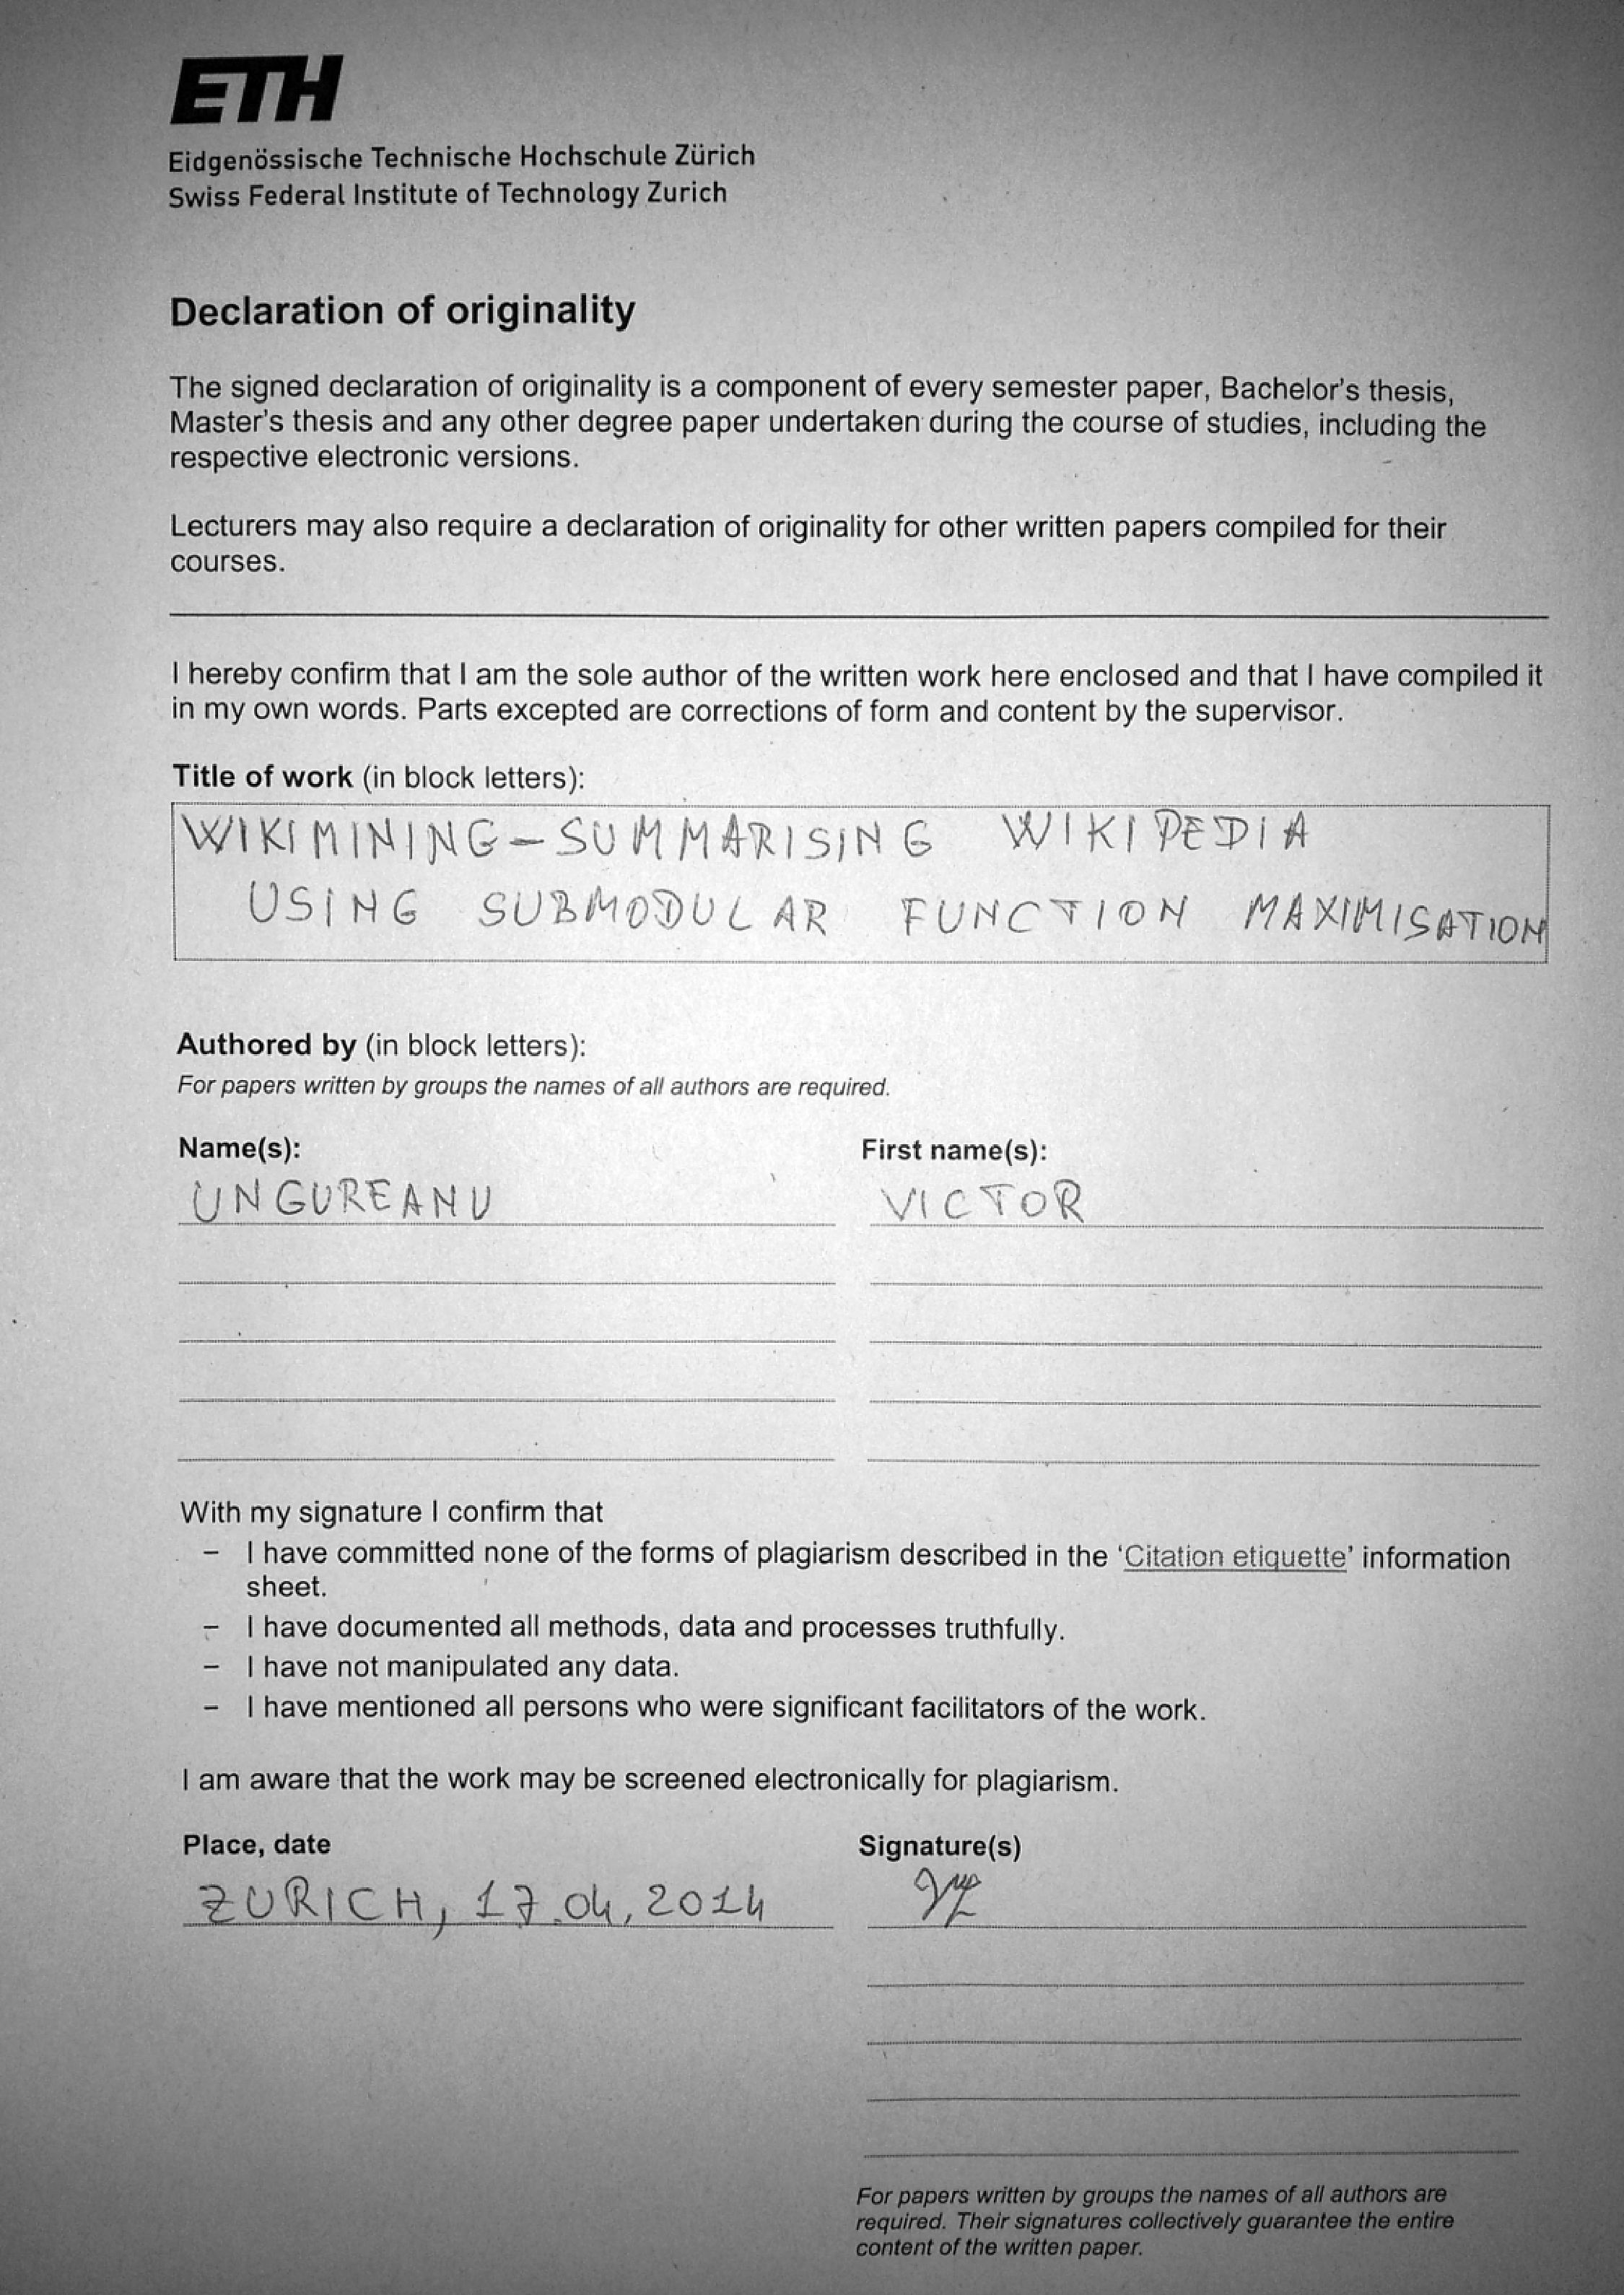
\includepdf[pages={1}]{images/declaration.pdf}

\end{document}
